\begin{surferPage}[Kummer]{Het vierdegraadsoppervlak van Kummer}
    In 1875 was Eduard Kummer de eerste die expliciet de vraag stelde wat het maximaal aantal singulariteiten $\mu(d)$ zou zijn in het geval van een oppervlak van de vierde graad.
  
  Hij bewees eerst dat $\mu(4)=16$, en daarna bestudeerde hij expliciet de vierdegraadsoppervlakken met exact 16 singulariteiten.
    Een bijzonder mooie familie van dergelijke oppervlakken wordt gegeven door:
    \[\bigl(x^2+y^2+z^2-\mu^2\bigr)^2 - \lambda
    \,y_0\,y_1\,y_2\,y_3,\]
    waar $\mu$ een vrije parameter is, en 
    $\lambda = \frac{3\mu^2-1}{3-\mu^2}$; de $y_i$ worden als zijden van een regelmatige tetra\"eder gekozen, daar het oppervlak symmetrisch is: {\small
    $y_0=1-z-\sqrt{2}x$, \  
    $y_1=1-z+\sqrt{2}x$, \ 
    $y_2=1+z+\sqrt{2}y$, \ 
    $y_3=1+z-\sqrt{2}y$}.
    
  Niet alle leden van deze familie hebben exact $16$ re\"ele singulariteiten,
  maar de meeste wel:
  \begin{center}
    \vspace*{-0.2cm}\hspace*{-0.2cm}
    \begin{tabular}{@{}c@{\,}c@{\,}c@{\,}c@{\,}c@{}}
      \begin{tabular}{@{}c@{}}
        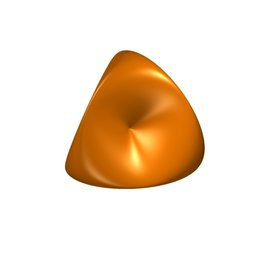
\includegraphics[height=1.4cm]{./../../common/images/kummer_0}
      \end{tabular}
      &
      \begin{tabular}{@{}c@{}}
        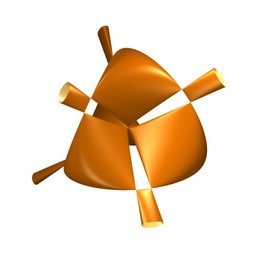
\includegraphics[height=1.4cm]{./../../common/images/kummer_1}
      \end{tabular}
      &
      \begin{tabular}{@{}c@{}}
        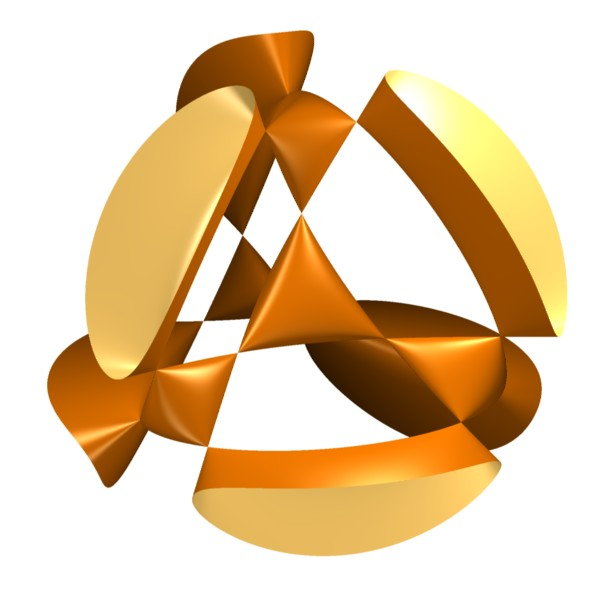
\includegraphics[height=1.4cm]{./../../common/images/kummer_2}
      \end{tabular}
      &
      \begin{tabular}{@{}c@{}}
        
\includegraphics[height=1.4cm]{./../../common/images/kummer_3}
      \end{tabular}
    \end{tabular}
  \end{center}
  \vspace{-0.2cm}  
   Voor enkele bijzondere waarden van de parameters kunnen verschillende singulariteiten samenvallen.
\end{surferPage}
